\cotefile{67}
\scanpage{2}

Chirurgie des \unsure{surfaces} conformes ---

1978 ou 77 ?)

% archive sheet number: 1
\scanpage{3}

Chirurgie des surfaces conformes.

1) \uline{Découpage} : Découpe d'une surface conforme \deleted{\unsure{(sans bord|(avec bord}} (évt avec bord) suivant un sous-1-complexe rectifiable compact : On trouve une surface conforme à \deleted{\illegible{1}} bord, avec morceau \inserted{\deleted{compact}} de bord compact marqué.

2) \uline{Recollage} : À partir d'une surface conforme (avec bord \deleted{\unsure{à recoller|non vide}}) et d'un morceau compact de bord, et une relation d'équivalence ``admissible'' \inserted{(au sens rectifiable)} sur le bord, \deleted{\unsure{au sens}} on trouve une surface conforme avec bord...

3) \uline{Rétrécissage}
\[
\underset{\substack{\text{1-compl.}\\\text{cpt}}}{K}\subset
\underset{\text{s. conforme avec bord}}{X},
\]
$\widetilde X$ découpé de $X$ suivant $K$, $\partial'\widetilde X$ partie distinguée du bord, on choisit un \inserted{multi}anneau autour de $\partial'\widetilde X$, \deleted{soit alors} (un germe de tel anneau autour d'une composante $(\partial'_{\unsure{i}}\widetilde X)_i$ revient : la donnée d'une structure Riemannienne \deleted{\unsure{régulière}} \inserted{rectifiable} de long. totale 1 sur celle-ci....)

\figure{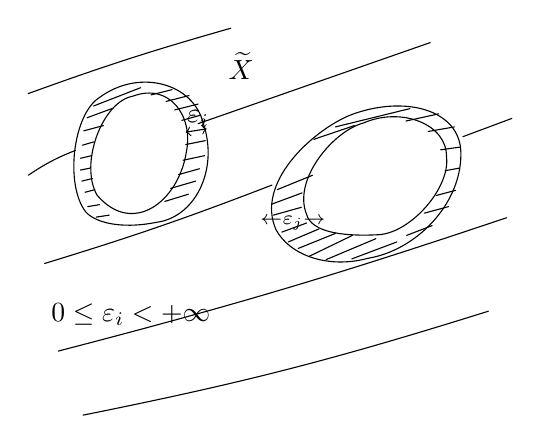
\begin{tikzpicture}[x=0.83cm,y=0.83cm,line cap=round,line join=round]
\draw[thin] (-0.6,2.5) to[bend left=2] (2.5,3.5);
\draw[thin] (-0.6,1.25) to[bend left=6] (0.12,1.63) (2.0,2.04) -- (5.55,3.28);
\draw[thin] (-0.35,-0.10) to[bend right=2] (3.13,1.10) (6.05,1.84) -- (6.80,2.12);
\draw[thin] (-0.14,-1.44) to[bend right=2] (6.72,0.60);
\draw[thin] (0.24,-2.42) to[bend right=3] (6.44,-0.83);
\draw (0.28,0.69) .. controls (-0.04,1.10) and (0.08,2.18) .. (0.49,2.44)
 .. controls (1.10,2.89) and (1.93,2.66) .. (2.08,2.04)
 .. controls (2.32,1.32) and (1.94,0.60) .. (1.36,0.53)
 .. controls (0.81,0.42) and (0.42,0.53) .. (0.28,0.69) -- cycle;
\draw (0.45,0.95) .. controls (0.18,1.44) and (0.54,2.38) .. (1.00,2.46)
 .. controls (1.56,2.67) and (1.93,2.16) .. (1.82,1.61)
 .. controls (1.70,0.84) and (0.99,0.31) .. (0.45,0.95) -- cycle;
\draw[thin] (0.40,2.31)--(1.12,2.59) (0.30,2.13)--(0.68,2.27) (0.25,1.93)--(0.55,2.01)
 (0.23,1.71)--(0.40,1.76) (0.20,1.51)--(0.37,1.55) (0.20,1.33)--(0.35,1.36)
 (0.22,1.16)--(0.38,1.20) (0.27,0.99)--(0.42,1.03) (0.31,0.77)--(0.49,0.80)
 (0.44,0.61)--(0.64,0.64) (1.28,2.48)--(1.60,2.56) (1.51,2.38)--(1.86,2.47)
 (1.64,2.25)--(2.00,2.34) (1.75,2.09)--(2.04,2.17) (1.81,1.72)--(2.11,1.78)
 (1.77,1.48)--(2.10,1.55) (1.70,1.26)--(2.02,1.35) (1.58,1.05)--(1.96,1.16)
 (1.49,0.85)--(1.85,0.96);
\draw[<->] (1.81,1.91)--(2.13,1.96);
\node[above,inner sep=0pt] at (2,1.98) {$\varepsilon_i$};
\node at (2.66,2.92) {$\widetilde X$};
\draw (3.19,0.42) .. controls (2.88,1.12) and (3.71,1.90) .. (4.30,2.16)
 .. controls (5.13,2.49) and (6.03,2.27) .. (6.02,1.57)
 .. controls (6.02,0.80) and (5.33,0.10) .. (4.60,-0.02)
 .. controls (3.97,-0.19) and (3.39,0.04) .. (3.19,0.42) -- cycle;
\draw (3.66,0.65) .. controls (3.44,1.18) and (4.07,1.93) .. (4.53,2.05)
 .. controls (5.10,2.30) and (5.81,2.04) .. (5.80,1.53)
 .. controls (5.86,1.06) and (5.25,0.36) .. (4.75,0.34)
 .. controls (4.14,0.31) and (3.73,0.40) .. (3.66,0.65) -- cycle;
\draw[thin] (3.21,1.03)--(3.75,1.25) (3.13,0.81)--(3.59,0.98) (3.15,0.64)--(3.58,0.76)
 (3.28,0.38)--(3.66,0.52) (3.38,0.23)--(3.85,0.43) (3.53,0.13)--(4.10,0.36)
 (3.70,0.01)--(4.36,0.33) (3.96,-0.04)--(4.72,0.28) (4.35,-0.03)--(5.04,0.23)
 (5.19,0.33)--(5.58,0.48) (5.46,0.67)--(5.83,0.77) (5.64,0.94)--(5.94,1.02)
 (5.78,1.32)--(6.00,1.36) (5.71,1.64)--(6.00,1.68) (5.52,1.92)--(5.92,1.99)
 (5.18,2.08)--(5.68,2.19) (4.10,1.99)--(5.24,2.27) (3.77,1.80)--(4.39,2.01);
\node[inner sep=0pt] at (3.45,0.52) {$\scriptstyle\leftarrow\varepsilon_j\rightarrow$};
\node at (0.97,-0.88) {$0\leq\varepsilon_i<+\infty$};
\end{tikzpicture}}

$\widetilde X^*$ la surface \inserted{à bord \deleted{\unsure{décrit}} \deleted{\unsure{défini}} \unsure{dite}} rétrécie déduite de la connue choisissons un isomorphisme rectifiable $\partial'\widetilde X^*\xrightarrow{\sim}\partial'\widetilde X$ compatible avec les comp. connexes, et utilisons la relation d'équivalence \inserted{de \unsure{recollement|recollage}} sur $\partial'\widetilde X$ pour en déduire une sur $\widetilde X^*$. On en conclut \deleted{$\unsure{K}$} $X^*$ et $K\subset X^*$

% archive sheet number: 2
\scanpage{4}

4) \uline{Élargissage} Opération inverse -- au lieu de retrancher une couronne, on en rajoute une...

5) Opération mixte : \uline{panachage}

On considère un voisinage tubulaire \unsure{'standart'|'standard'} de $\partial'\widetilde X$, et dans \inserted{chaque composante $T_i$ de} celui-ci, un cercle $\Gamma_i$, et un isom. rect. $\Gamma_i\simeq(\partial'\widetilde X)_i$. On \deleted{\unsure{se donne}} \inserted{\deleted{définit}} \deleted{considère}\inserted{considère} $\deleted{\unsure{\partial}}\widetilde X^*$ déduit de $\widetilde X$ en enlevant \inserted{$\forall i$} ``la \deleted{\unsure{intérieur|intérieure}'' de $\Gamma_i$} partie de $T_i$ '' entourée par $\Gamma_i$ ''. On termine comme dans 3°), 4°) pour former $\widetilde X^*$ et $K\subset X^*$.

\figure{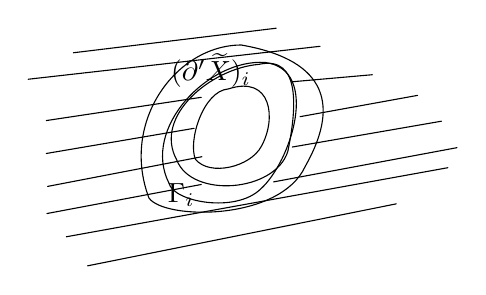
\begin{tikzpicture}[x=0.82cm,y=0.82cm,line cap=round]
\draw[thin] (-2.7,2.28)--(0.44,2.66) (-3.4,1.87)--(1.12,2.38)
 (-3.12,1.23)--(-0.72,1.59) (0.68,1.83)--(1.93,1.94)
 (-3.12,0.72)--(-0.83,1.11) (0.81,1.29)--(2.63,1.62)
 (-3.10,0.21)--(-0.71,0.67) (0.69,0.82)--(3.00,1.22)
 (-3.11,-0.21)--(-0.72,0.24) (0.40,0.28)--(3.24,0.81)
 (-2.81,-0.57)--(3.10,0.50) (-2.48,-1.02)--(2.30,-0.06);
\draw (-1.53,0.03) .. controls (-1.98,1.22) and (-1.10,2.40) .. (-0.10,2.40)
 .. controls (1.10,2.19) and (1.49,1.58) .. (0.89,0.52)
 .. controls (0.50,-0.33) and (-1.29,-0.31) .. cycle;
\draw (-1.22,0.26) .. controls (-1.65,1.11) and (-0.61,2.19) .. (0.27,2.13)
 .. controls (1.13,2.02) and (0.67,0.59) .. (0.20,0.17)
 .. controls (-0.19,-0.21) and (-1.15,-0.03) .. cycle;
\draw (-1.10,0.62) .. controls (-1.47,1.30) and (-0.56,2.04) .. (0.17,2.10)
 .. controls (0.84,2.25) and (0.75,1.38) .. (0.62,0.75)
 .. controls (0.42,0.12) and (-0.87,0.02) .. cycle;
\draw (-0.81,0.63) .. controls (-0.93,0.91) and (-0.69,1.69) .. (-0.30,1.72)
 .. controls (0.37,1.94) and (0.45,1.26) .. (0.21,0.83)
 .. controls (0.04,0.51) and (-0.59,0.36) .. cycle;
\node at (-0.57,2.00) {$ (\partial'\widetilde X)_i $};
\node at (-1.03,0.08) {$\Gamma_i$};
\end{tikzpicture}}
% slanted
\margin{C'est une composition rétrécissage $\circ$ élargissage, ou mieux élargissage $\circ$ rétrécissage.}

\unsure{4°)|4 bis)|5°)|4')} \uline{Commutation} de l'opération de panachage relative à diverses composantes connexes de $K$.

6) Cas d'une composante \inserted{$C$} de $K$ boucle isolée \inserted{plongée $\mathbb R$-analytique}. L'opération de panachage revient alors tjrs à une composition de 1) enlever une couronne \inserted{$\mathbb R$-analytique} autour de $C$ 2°) Recoller \inserted{$\mathbb R$-analytiq\textsuperscript{mt}} par un cylindre les deux bords \inserted{\unsure{qui restent|jointifs|joints}} de la couronne enlevée....

\figure{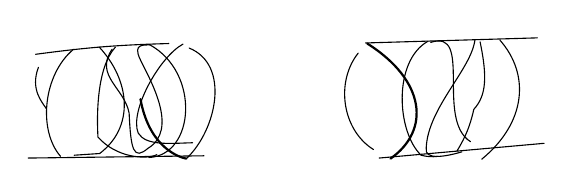
\begin{tikzpicture}[x=0.72cm,y=0.72cm,line cap=round]
\draw (0,0)--(3.1,0.04) (0.13,1.83) to[bend left=3] (2.48,2.02);
\draw (0.80,1.92) .. controls (0.26,1.47) and (0.17,0.49) .. (0.57,0.03);
\draw[thin] (0.18,1.60) .. controls (0.03,1.21) and (0.25,0.98) .. (0.32,0.87);
\draw (1.54,1.96) .. controls (1.20,1.59) and (1.21,0.72) .. (1.23,0.37) .. controls (1.56,0) and (2.08,-0.03) .. (2.27,0.06);
\draw[thin] (1.25,1.96) .. controls (1.80,1.37) and (1.88,0.55) .. (1.26,0.08)--(0.81,0.05);
\draw (1.48,1.92) .. controls (1.16,1.45) and (1.70,1.24) .. (1.78,0.79) .. controls (1.81,0.13) and (1.86,-0.04) .. (2.11,0.17)
 .. controls (2.66,0.50) and (2.16,1.36) .. (1.98,1.73) .. controls (1.82,2.05) and (2.08,1.98) .. (2.15,2.00);
\draw (2.14,2.0) .. controls (3.04,1.51) and (2.94,0.05) .. (2.13,0.01);
\draw (2.73,2.01) .. controls (2.32,1.79) and (1.78,0.83) .. (1.94,0.44) .. controls (2.08,0.21) and (2.50,0.26) .. (2.90,0.27);
\draw[thick] (1.98,1.04) .. controls (2.12,0.26) and (2.58,0.03) .. (2.79,-0.01);
\draw (2.84,1.94) .. controls (3.57,1.64) and (3.32,0.50) .. (2.80,0.00);
\begin{scope}[shift={(5.9,0)}]
\draw (0.05,2.03)--(3.08,2.12) (0.29,0.00)--(3.20,0.26);
\draw[thin] (-0.08,1.85) .. controls (-0.48,1.35) and (-0.37,0.50) .. (0.19,0.15);
\draw[thick] (0.08,2.02) .. controls (1.11,1.37) and (1.20,0.49) .. (0.49,-0.01);
\draw (1.15,2.06) .. controls (0.53,1.71) and (0.60,0.46) .. (1.03,0.05) to[bend right=10] (1.33,0.03);
\draw[thin] (1.20,2.04) .. controls (1.95,2.29) and (1.28,0.68) .. (1.90,0.29);
\draw (1.98,2.09) .. controls (1.92,1.57) and (1.15,0.89) .. (1.12,0.18) .. controls (1.08,-0.05) and (1.48,0.03) .. (1.75,0.11);
\draw (2.07,2.05) .. controls (2.20,1.43) and (2.18,1.10) .. (1.96,0.86) to[bend left=9] (1.66,0.12);
\draw[thin] (2.42,2.08) .. controls (2.95,1.48) and (2.89,0.63) .. (2.10,-0.02);
\end{scope}
\end{tikzpicture}}

\deleted{\figure{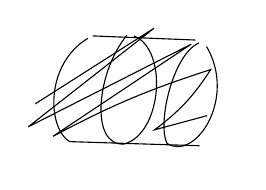
\begin{tikzpicture}[x=0.75cm,y=0.75cm]
\draw (0.37,1.66) .. controls (-0.37,1.21) and (-0.31,0.13) .. (0.06,-0.09) -- (2.26,-0.16);
\draw (0.45,1.70)--(2.19,1.63);
\draw (1.03,1.71) .. controls (0.51,1.08) and (0.40,-0.18) .. (0.99,-0.13) .. controls (1.63,0.06) and (1.73,1.47) .. (1.15,1.70);
\draw (2.25,1.58) .. controls (1.81,1.39) and (1.54,0.22) .. (1.71,-0.12) .. controls (2.18,-0.43) and (2.90,0.63) .. (2.38,1.52);
\draw (-0.52,0.55)--(1.49,1.83)--(-0.64,0.16)--(2.12,1.56)--(-0.22,0.00) to[bend left=5] (2.45,1.13) to[bend right=-10] (1.50,0.11)--(2.39,0.35);
\end{tikzpicture}}}

relations avec les \deleted{\unsure{deux|de}} \inserted{petits} \unsure{plong\textsuperscript{mts}|plongements|plongés} conformes d'une petite couronne...

% archive sheet number: 3
\scanpage{5}

7) Modules pour $S\subset K\subset X$

On suppose \inserted{\deleted{$X$} compacte, et} pour simplifier $X$ \deleted{compacte} \inserted{sans bord} orientée. Ceci dit, on fixe $S_0\subset K_0\subset X_0$ situation top, et on \uline{rigidifie} $(S\subset K\subset X)$ en se donnant une classe d'isotopie d'\unsure{hom.|isom.|homéo.} top. avec la situation standart. On élimine ainsi les autos, sauf dans le cas \deleted{$\unsure{X_0|K_0|X}$} où $X_0$ a des composantes de degré $0,1$.....

Pour avoir un ``\unsure{nb|ens} fini de modules'', on \inserted{pourrait} exiger \inserted{p. ex.} que les arêtes de $K$ soient des arcs de cercles pour la conn. projective canonique. Mais les ``cartes \inserted{cell.} holomorphes'' ne satisfont pas néc. à cette condition ! On pourrait exiger plutôt que pour \deleted{\unsure{une|ces|avec}} les : paramétrisations géodésiques sur la découpe, sur disques \unsure{que|orc|avec} l'\unsure{homéomorphisme|homographie|isomorphisme} de recollement soit linéaire. [Éventuelt on pourrait exiger l'équidistance \inserted{des sommets} sur chaque composante connexe du bord de la découpe...] Mais on a des ennui pour les morceaux \deleted{de genre 0} \inserted{qui sont des disques \unsure{non ponctués|monoponctués}} il n'y a pas de métrique \unsure{inst courb $-$|intrinsèque|constant}. Il

% archive sheet number: 4
\scanpage{6}

\[
\begin{aligned}
&\deleted{\widetilde L_0=\pi^{-1}(L_0)\subset\widetilde K_0}\\
&\deleted{\widetilde L=T}
\end{aligned}
\]
\diagram{\begin{tikzcd}[ampersand replacement=\&,row sep=0.1em,column sep=1em]
\widetilde K \arrow[rr,"\pi"] \& \& K\\
\cup \& \& \deleted{\unsure{\cup}}\quad\unsure{\supset}\\
\widetilde L \& {}=\pi^{-1}(L)\arrow[r] \& L
\end{tikzcd}}

\[
\left\{\begin{aligned}
|\widetilde K|-|\widetilde L|&\xrightarrow{\sim}|K|-|L|\\
(\widetilde K,\widetilde L)&\text{ est ``pur''}
\end{aligned}\right.
\qquad
\widetilde K=\varinjlim_{x\in K\backslash L}
\underset{\substack{\shortparallel\\ \{y\in K\mid y\leq x\}}}{K_x}
\]

\figure{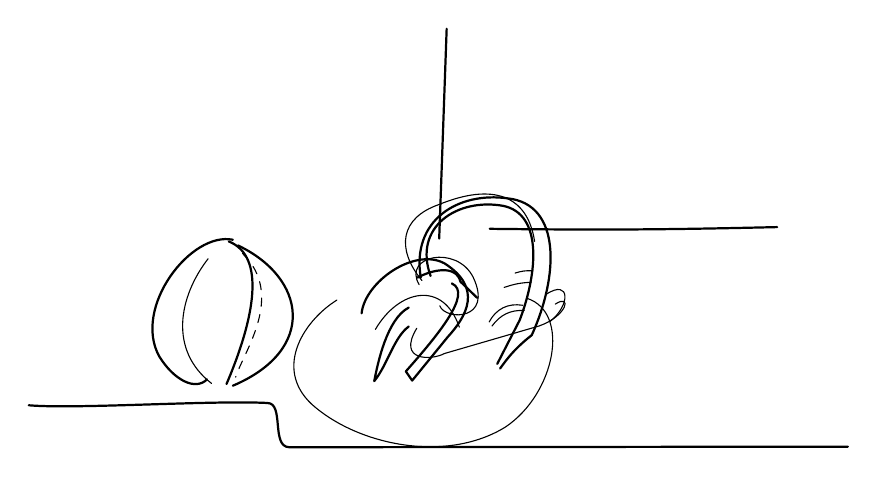
\begin{tikzpicture}[x=0.73cm,y=-0.73cm,line cap=round,line join=round]
\draw[thick] (0.0,2.98) .. controls (0.81,3.05) and (3.19,2.89) .. (4.15,2.94)
 .. controls (4.45,2.94) and (4.21,3.70) .. (4.53,3.71) -- (14.25,3.70);
\draw[thick] (8.02,-0.09) to[bend right=1] (13.02,-0.12);
\draw[thick] (7.27,-3.57)--(7.14,0.08);
\draw[thick] (3.55,0.10) .. controls (2.82,-0.05) and (1.80,1.28) .. (2.27,2.13)
 .. controls (2.53,2.55) and (2.90,2.73) .. (3.10,2.53);
\draw (3.12,0.43) .. controls (2.61,1.09) and (2.43,2.02) .. (3.18,2.60);
\draw[thick] (3.48,0.13) .. controls (4.13,0.39) and (3.93,1.46) .. (3.44,2.61);
\draw[thin,dashed] (3.72,0.34) .. controls (4.47,1.07) and (3.73,2.06) .. (3.60,2.49);
\draw[thick] (3.64,0.20) .. controls (4.82,0.76) and (5.03,2.01) .. (3.55,2.64);
\draw (5.36,1.15) .. controls (4.75,1.53) and (4.23,2.40) .. (4.99,3.02)
 .. controls (5.80,3.69) and (7.28,3.98) .. (8.29,3.36)
 .. controls (9.16,2.78) and (9.43,1.37) .. (8.67,1.12);
\draw[thick] (5.79,1.38) .. controls (5.85,0.83) and (6.71,0.23) .. (7.23,0.51)
 .. controls (7.91,0.94) and (7.61,1.44) .. (7.29,1.79) -- (6.67,2.55)--(6.56,2.39)
 .. controls (7.10,1.78) and (7.73,1.03) .. (7.36,0.86);
\draw (6.03,1.66) .. controls (6.44,0.96) and (7.21,0.80) .. (7.49,1.62);
\draw[thick] (6.61,1.28) .. controls (6.23,1.48) and (6.07,2.25) .. (6.01,2.56)
 .. controls (6.25,2.26) and (6.35,1.80) .. (6.61,1.61);
\draw (6.75,1.64) .. controls (6.40,2.22) and (7.01,2.20) .. (7.23,2.08) -- (8.88,1.60)
 .. controls (9.38,1.42) and (9.45,1.03) .. (9.16,1.22);
\draw (6.79,0.88) .. controls (6.50,0.38) and (7.44,0.18) .. (7.73,0.75)
 .. controls (8.09,1.51) and (7.25,1.51) .. (7.15,1.25);
\draw[thick] (6.76,0.76) .. controls (7.00,0.63) and (7.43,0.52) .. (7.51,0.83)--(7.80,1.11);
\draw[thin] (6.84,0.81) .. controls (6.38,0.25) and (6.47,-0.28) .. (7.13,-0.51)
 .. controls (8.08,-0.90) and (8.68,-0.67) .. (8.80,0.13);
\draw[thick] (6.82,0.76) .. controls (6.65,-0.24) and (7.47,-0.74) .. (8.33,-0.62)
 .. controls (9.27,-0.52) and (9.22,0.73) .. (8.75,1.76) to[bend right=8] (8.20,2.34);
\draw[thick] (6.99,0.73) .. controls (6.68,-0.13) and (7.46,-0.63) .. (8.25,-0.49)
 .. controls (8.95,-0.35) and (8.85,0.69) .. (8.54,1.50) -- (8.15,2.26);
\draw (8.01,1.53) to[bend left=36] (8.59,1.24) (8.06,1.60) to[bend left=28] (8.62,1.33)
 (8.27,0.93) to[bend left=8] (8.74,0.84) (8.46,0.68) to[bend left=10] (8.77,0.64)
 (9.00,1.05) .. controls (9.43,0.77) and (9.42,1.25) .. (9.07,1.52);
\end{tikzpicture}}
% crop-candidate: scan 6

% slanted
\margin{$\begin{aligned}
|x'|,|y'|&\leq\sqrt{x^{\prime\unsure{2}}\unsure{+|-}y^{\prime 2}}\leq |x'|+|y'|\\
\int|x'|,\int|y'|&\leq\int -\leq\int|x'|+\int|y'|
\end{aligned}$}

\[
\sum_{\widetilde K_i}(X_i,\partial X_i)=|\widetilde K_i|
\]

\figure{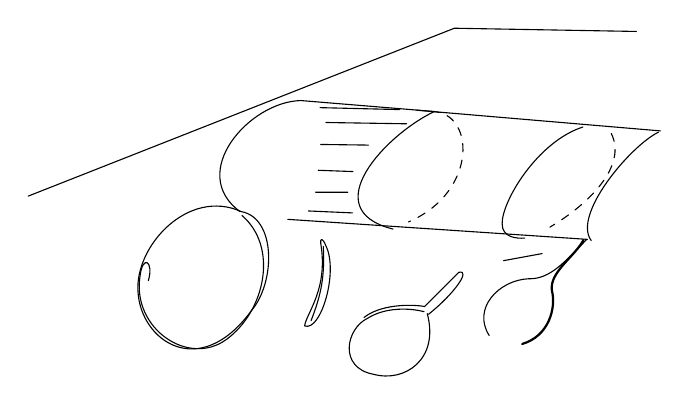
\begin{tikzpicture}[x=0.82cm,y=-0.82cm,line cap=round,line join=round]
\draw[thin] (0,2.35)--(6.6,-0.25)--(9.42,-0.20);
\draw[thin] (3.28,2.59) .. controls (2.46,1.99) and (3.42,0.89) .. (4.22,0.87)
 --(6.29,1.04) .. controls (5.55,1.39) and (4.43,2.56) .. (5.65,2.86);
\draw (4.02,2.71) --(8.66,3.02) (6.02,1.02)--(9.79,1.34);
\draw (8.59,1.28) .. controls (7.88,1.51) and (7.33,2.44) .. (7.34,2.78)
 .. controls (7.34,2.99) and (7.56,3.01) .. (7.69,3.00);
\draw (9.76,1.36) .. controls (9.33,1.57) and (8.42,2.64) .. (8.72,3.04);
\draw[dashed,thin] (6.24,1.04) .. controls (6.92,1.03) and (6.98,2.28) .. (5.89,2.75)
 (9.03,1.38) .. controls (9.28,1.88) and (8.69,2.47) .. (8.08,2.83);
\draw[thin] (4.52,0.98)--(5.75,1.01) (4.61,1.21)--(5.86,1.23) (4.53,1.55)--(5.27,1.56)
 (4.49,1.95)--(5.03,1.97) (4.45,2.29)--(4.95,2.29) (4.34,2.58)--(5.02,2.61);
\draw (3.30,2.59) .. controls (3.84,2.69) and (3.83,3.68) .. (3.46,4.12)
 .. controls (2.65,5.23) and (1.74,4.59) .. (1.70,3.83) .. controls (1.65,3.12) and (2.48,2.22) .. cycle;
\draw[thin] (3.31,2.65) .. controls (3.88,3.14) and (3.67,4.13) .. (3.07,4.57)
 .. controls (2.48,5.00) and (1.61,4.40) .. (1.73,3.60) .. controls (1.77,3.24) and (1.95,3.36) .. (1.86,3.66);
\draw (4.53,3.08) .. controls (4.65,3.79) and (4.31,4.16) .. (4.28,4.36)
 .. controls (4.53,4.46) and (4.81,3.52) .. (4.61,3.12) .. controls (4.56,2.99) and (4.52,3.00) .. cycle;
\draw[thin] (4.57,3.13) to[bend left=12] (4.38,4.28);
\draw (5.20,4.23) .. controls (5.45,4.03) and (5.91,4.02) .. (6.14,4.06)
 --(6.67,3.53) .. controls (6.86,3.49) and (6.60,3.86) .. (6.20,4.18);
\draw (6.18,4.17) .. controls (6.37,4.88) and (5.83,5.24) .. (5.35,5.11)
 .. controls (4.80,5.01) and (4.92,4.40) .. (5.26,4.24) .. controls (5.53,4.07) and (5.90,4.08) .. (6.13,4.14);
\draw (7.14,4.51) .. controls (6.87,4.09) and (7.29,3.65) .. (7.75,3.63)
 .. controls (8.08,3.64) and (8.31,3.37) .. (8.65,3.02);
\draw[thick] (7.65,4.64) .. controls (8.06,4.52) and (8.18,4.09) .. (8.11,3.81)
 .. controls (8.07,3.53) and (8.46,3.29) .. (8.60,3.03);
\draw (7.36,3.35)--(7.96,3.24);
\end{tikzpicture}}
% crop-candidate: scan 6
% archive sheet number: 5
\scanpage{7}

vaut mieux dès lors exiger que ces \unsure{isos|arêtes} soient \uline{homographiques} par morceaux....

Dans le premier cas (exigeant que les disques de la découpe soient poncturés...) on trouve, en supposant $\pi_0(K_0)\longrightarrow\pi_0(X_0)$ surjectif, \deleted{et quitte \unsure{à éliminer} des bords isolés....}
\[
\text{nb de modules \inserted{réels}}\quad N=\left(\sum_{\substack{f\in\pi_0(X\backslash K)=F\\f\text{ pas \uline{un} disque}}}
(6g(f)+4\nu(f)\deleted{\unsure{+}}-6)\right)\deleted{+\unsure{\mu}}
\]
\deleted{$\mu$ étant le nb de ``faces'' $f$ qui sont des \deleted{disques}\inserted{\unsure{anneaux|couronnes}}.}

$\checkmark/$ si $g\ge 2$

\margin{On suppose $X_0^0$ connexe ainsi que $K$ aussi. $\lambda$ la connexité de $K$}
\[
\begin{aligned}
3g-3\qquad\text{où}\quad 2-2g&=\chi=\sum_{f\in F}\bigl(2-2g(f)-\nu(f)\bigr)\\
&\hspace{8em}+1-\lambda\\
\text{i.e.}\qquad 2g-2&=\sum_{f\in F}\bigl(2g(f)-2+\nu(f)\bigr)\\
&\hspace{8em}+(\lambda-1)\\
g-1&=\tfrac12\sum_{f\in F}\bigl[2g(f)-2+\nu(f)-\bigr]\\
&\hspace{8em}+\tfrac{\unsure{3|1}}2(\lambda-1)\\
3(g-1)&=\tfrac32\sum_{f\in F}\bigl[2g(f)-2+\nu(f)\bigr].\\
&\hspace{8em}+\tfrac32(\lambda-1)\\
&=\sum_{f\in F}\bigl[3(g(f)-1)+\tfrac32\deleted{\unsure{2}}\nu(f)\bigr]\\
&\hspace{8em}+\tfrac32(\lambda-1)
\end{aligned}
\]
\[
(g\ge2)\qquad N-(3g-3)=\sum_{\substack{f\in F\\f\text{ pas un disque}}}
\bigl(3g(f)+\tfrac52\nu(f)-3\bigr)\deleted{\unsure{-}}+
\deleted{\sum_{\substack{f\in F\\f\ \mathrm{disque}}}\unsure{1}}
\tfrac32(\mu+\unsure{1-\lambda})\overset{?}{\ge}0
\]
$\mu$ étant le nb de $f$ qui sont des disques
\[
(g=1)\qquad N-1=\sum_{\substack{f\ \text{pas un}\\\text{disque}\\\text{[NB }g(f)=0\ \text{tjrs]}}}
(\underbrace{4\nu(f)-6}_{\geqslant 2})-1
\]
% archive sheet number: 6
\scanpage{8}

\deleted{LISTE DE TERRAINS\\
-=-=-=-=-=-=-=-=-=-=-}

\deleted{Réf. 2 \quad LODEVE \quad 2.450 M2 E.E.E. Expo. Est - vigne - route - \quad Prix : 90.000 Frs}

\deleted{Réf. 5 VERNAZOUBRES \quad 4.750 M2 E.E. \quad Expo. Ouest - c\unsure{\^{h}|h}êne - pin - route - \quad Prix : 13.000 Frs}

\deleted{Réf. 7 VERNAZOUBRES 161.640 M2 \uline{très isolé} \quad expo. Ouest - chemin \quad Prix : 90.000 Frs}

\deleted{Réf. 11 LE LEZ \quad 5.000 M2 E.E. \quad expo. Sud - pinède - accès chemin Prix : 60.000 Frs}

\deleted{Réf. 13 LACOSTE \quad 11.000 M2 E.E. \quad Expo. Ouest - boisé - chemin \quad Prix : 98.000 Frs}

\deleted{Réf. 14 LACOSTE \quad 13.390 M2 E.E.E. Expo. Sud - vigne - bois - \quad Prix : 70.000 Frs}

\deleted{Réf. 15 VERNAZOUBRES 23.000 M2 Source Expo. Ouest - boisé - Isolé - chemin \quad Prix : 24.000 Frs}

\deleted{Réf. 20 CAUX \quad Lotissement de 590 à 640 M2 entièrement terminé - \quad Prix : 43.000 à 48.000\unsure{Nrs|Frs}}

\deleted{Réf. 32 LACOSTE \quad 1.000 M2 E.E. \quad Expo. Ouest - ancien jardin dans village \quad Prix : 42.000 Frs -}

\deleted{Réf. 33 FOZIERES \quad 4.000 M2 E.E. \quad Expo. Est - boisé et arbres fruitiers - chemin - Prix 35.000 F}

\deleted{Réf. 34 ARBORAS \quad 22.500 M2 Beau point de vue - Expo. Ouest - vigne- 2.500 M2 solde bois - chemin - Prix : 20.000 Frs}

\deleted{Réf. 36 ARBORAS \quad 4.000 M2 E.E. beau point de vue - expo. Ouest - chemin - oliviers - Prix : 26.000F}

\deleted{Réf. 55 ST ETIENNE G. 6.000 M2 Elect. Expo. Sud - boisé - accès par deux chemins \quad Prix : 40.000 Frs}

\deleted{Réf. 57 VILLENEUVETTE 15.000 M2 E.E. Téléph. Expo. Est - ancienne vigne- chemin - \quad Prix : 70.000 Frs}

\deleted{Réf. 65 ST ETIENNE G. \quad 5.000 M2 E.E. Expo. Est - jolie vue s/village - \quad Prix : 50.000 Frs}

\deleted{Réf. 69 ST ETIENNE G. \quad 7.141 M2 E.E. Expo. Ouest - oliviers - vigne - chemin \quad Prix : 35.000 Frs}

.../...
% archive sheet number: 7
\scanpage{9}

\textcircled{1} courbe ell.\unsure{pt|1|$X$} $+$ géod. fermée \uline{orientée} $\gamma$

\textcircled{2} \deleted{courbe}. \inserted{groupe} elliptique $X_{\unsure{0|*}}+$ \deleted{\unsure{ss tore|sa jac.} \unsure{réel|relle} \inserted{\unsure{de sa}} $\unsure{\mathbb U_0|\mathbb U}$}
$\displaystyle\underset{X_0(\mathbb C)}{\downarrow}$

$+\ \unsure{\mathbb U_0|\mathbb U}-\text{torseur}\ \gamma$

\textcircled{3} $X_0+\deleted{\unsure{Z}}\unsure{\alpha|a}\subset\unsure{H|\pi}_1(X_0)+\Gamma$
\inserted{$\hookrightarrow$ primitif}

\textcircled{4} Torseur $\Gamma$ sous $\mathbb U$, et
$\begin{array}{c}Z\\[-2pt]\tikz[baseline=-.5ex]{\node[rotate=90,inner sep=0pt] {$\simeq$};}\\[-2pt]\mathbb Z\end{array}
\underset{\text{discret}}{\subset}\mathbb C^{*}$

\textcircled{5}

\textcircled{6}
% archive sheet number: 8
\scanpage{10}

% letterhead
\begin{center}
UNIVERSITE DES SCIENCES ET TECHNIQUES\\
DU LANGUEDOC\\
\rule{1cm}{0.2pt}\\
INSTITUT DE MATHEMATIQUES\\
Place Eugène Bataillon\\
34060 MONTPELLIER CEDEX
\end{center}

\handwritten{M. Grothendieck}

\figure{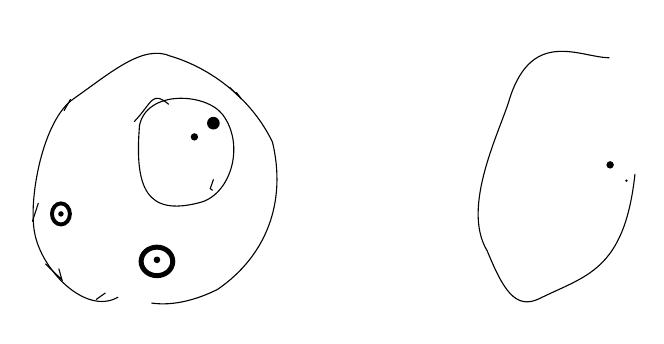
\begin{tikzpicture}[x=.67cm,y=.67cm,line cap=round]
\draw (1.6,.05) .. controls (.98,-.3) and (.14,.58) .. (.02,1.28)
 .. controls (-.1,1.9) and (.17,3.42) .. (.77,3.82)
 .. controls (1.48,4.32) and (2.08,4.85) .. (2.6,4.62)
 .. controls (3.38,4.39) and (4.15,3.79) .. (4.53,2.99)
 .. controls (4.8,1.86) and (4.42,.84) .. (3.49,.2)
 .. controls (3.11,.01) and (2.66,-.12) .. (2.24,-.06);
\draw (2.01,3.31) .. controls (2.15,3.98) and (3.25,3.93) .. (3.58,3.52)
 .. controls (4.03,2.93) and (3.73,1.97) .. (3.13,1.84)
 .. controls (2.15,1.59) and (1.91,2.11) .. (2.01,3.31);
\fill (3.41,3.35) circle (.12); \fill (3.05,3.09) circle (.07);
\draw[line width=1.4pt] (.52,1.63) ellipse (.17 and .2); \fill (.52,1.63) circle (.052);
\draw[line width=1.8pt] (2.34,.73) ellipse (.3 and .27); \fill (2.34,.76) circle (.063);
\draw (-.02,1.49)--(.09,1.83) (.23,.68)--(.54,.38)--(.48,.59)
 (1.19,.01)--(1.36,.13) (.58,3.59)--(.7,3.8)
 (3.72,4.03)--(3.94,3.81)--(3.85,3.93)
 (1.91,3.38)..controls (2.26,3.75) and (2.24,3.97)..(2.56,3.71)
 (3.41,2.28)--(3.35,2.11)--(3.39,2.08);
\draw (10.91,4.59)..controls (10.36,4.6) and (9.46,5.15)..(9.03,3.83)
 ..controls (8.86,3.23) and (8.09,1.77)..(8.6,.93)
 ..controls (8.9,.2) and (9.13,-.19)..(9.58,.02)
 ..controls (10.46,.46) and (11.2,.54)..(11.4,2.38);
\fill (10.93,2.56) circle (.07); \fill (11.24,2.26) circle (.025);
\end{tikzpicture}}
% archive sheet number: 9
\scanpage{11}

\textcircled{1} courbe elliptique $X+$ géod. fermée \uline{orientée} $\overline\Gamma$ \unsure{unit. tr.|mod. tr.}

\textcircled{2} \rule{1.6cm}{0.25pt} $X+$ \deleted{\unsure{ss-groupe} \unsure{tore|top.} \unsure{privilégié|algéb.} \unsure{réel}} $\mathbb U$ (tore cpt standard) $\subset X_0$

\textcircled{3} \rule{1cm}{0.25pt} $X+a\in\pi_1(X)$ élément primitif

\textcircled{4} ss. groupe discret $(\simeq\mathbb Z)$ \deleted{$Z\subset\mathbb C^*$}
\inserted{$Z\subset\mathbb C^*$ $(\Leftrightarrow b\in\mathbb C^*,\,0<|b|<1)$} et torseur $\Delta$ sous $\mathbb C^*$ \deleted{et $Z\subset\mathbb C^*$ discret}

\textcircled{5} Droite vector. \unsure{algébrique|élémentaire} $E$, \deleted{(d'où $\Delta=E^*$), et} \deleted{$\unsure{\{b,b^{-1}\}}\unsure{\leftrightarrow}b$} et $b\in\mathbb C\quad0<|b|<1$

(\uline{NB}\quad $\Delta=E^*,\ \deleted{\unsure{Z}}\ T=\mathbb G_{m}^*,\quad Z={}$ groupe engendré par $b$)
\[
P=\widehat E,\quad \{u,u^{-1}\}=\deleted{b,b^{-1}}\ \text{\unsure{hom.}}\ \{b,b^{-1}\}
\]

\textcircled{6} \deleted{forme $G$ de $\unsure{GP(1)|Gl(1)}_{\mathbb C}$}, $+$ \deleted{\unsure{élém.} \inserted{\deleted{tore}} de $G$} \inserted{couple de Killing} \deleted{Borel} $T\subset B\subset G$, \deleted{et $b\in B$ tel que} \inserted{\unsure{i.e.|g.i.e.} $G$ déduit}

\deleted{le groupe $b$}

de $\unsure{GP(1)|Gl(1)}_{\mathbb C}$ en tordant par un torseur sous $T\overset{\unsure{\mathrm{?}}}{\simeq}$ (\unsure{cas} $\mathbb G_m$ \uuline{can}) \inserted{i.e. torseur sous $\mathbb C^*$} [qui ne soit autre que $E^*$] enfin $Z\subset\deleted{T}\mathbb C^*=T(\mathbb C)$ ss groupe discret, (i.e. $Z$ déterminé par $b$) \quad $///\quad G\supset B\ni b$, avec $b$ \unsure{1/2 simple}

et $|b|$ (défini ind. près, \unsure{ou} : l'inverse) $\ne1$

\[
\deleted{\text{ens}}\ \underset{\text{\textcircled{1}}}{\{\Gamma\}}
\simeq\underset{\text{\textcircled{1}}}{X/\Gamma_0}
\simeq\underset{\text{\textcircled{3'}}}{X/\deleted{\mathbb Z}\mathbb R}
\simeq\deleted{\underset{\text{\textcircled{4}}}{\unsure{\Delta/\mathbb R_c}}}
{\Delta}/{(T_c\cdot Z)}
\simeq
\]
\inserted{\deleted{\unsure{ss groupe compact connexe}}}
\deleted{droites projectives P}
ens des \uline{cercles} de $P$ \deleted{admettant} admettant $\{u,u^{-1}\}$ comme bicentre \textcircled{5}
% archive sheet number: 10
\scanpage{12}

% letterhead
\begin{center}
UNIVERSITE DES SCIENCES ET TECHNIQUES\\
DU LANGUEDOC\\
\rule{1cm}{0.2pt}\\
INSTITUT DE MATHEMATIQUES\\
Place Eugène Bataillon\\
34060 MONTPELLIER CEDEX
\end{center}

\handwritten{Jean Pierre \unsure{Drij|Duij}}
% archive sheet number: 11
\scanpage{13}

\deleted{\unsure{corps de base|coupe de tore} $\mathbb C$}

\textcircled{1} courbe elliptique $X+$ géodésique fermée $\Gamma$ / mod. translation

$\Updownarrow$

\textcircled{2} courbe elliptique $X+$ \deleted{géodésique ferm.} \inserted{\deleted{\unsure{ss-groupe|s.-gpe} : 1 \unsure{par.}}} \unsure{comp.|i.e.}-tore réel $\Gamma_0$ de la courbe elliptique des $X_0$ \inserted{translation}

$\Updownarrow$

\textcircled{3} courbe elliptique $X+$ \deleted{\unsure{gén. élément} primitif de} \inserted{sous-groupe libre de rg 1 $Z\subset$} $\pi_1(X)$

$\Updownarrow$

\textcircled{4} forme \deleted{$\unsure{\mathbb G}$}\inserted{$T$} de $\mathbb G_m$, \inserted{sous-groupe \deleted{\unsure{fini}}\deleted{discret} libre rg 1} $Z\subset T(\mathbb C)$ \deleted{\unsure{non} $\unsure{|b|\ne1}$}, et torseur $\Delta$ sous $T$

\textcircled{4'} forme $T$ de $\mathbb G_m$, \deleted{et $u\in\mathbb C\ \unsure{[\,1,u^{-1}\,]}$} \inserted{$b\in\mathbb C\quad0<|b|<1$} et torseur $\Delta$ sous $T$

$\Updownarrow$

\textcircled{5} droite projective $P$, $+$ autom. $u$ de $P$ \inserted{couple $\{u,u^{-1}\}$ d'} non paraboliques (i.e. ayant 2 pts fixes distincts) et ayant des val. propres $\lambda,\lambda^{-1}$ tels que $|\lambda|\ne1$ (OBS, plutôt : \deleted{\unsure{distinct}} \inserted{\deleted{\unsure{prendre}}} \deleted{$\lambda,\lambda^{-1}$ \unsure{distincts}} que $|\lambda|>1$)

$\Updownarrow$

\textcircled{6} forme \inserted{$G$} de $\unsure{GP(1)|Gl(1)}_{\mathbb C}$, $+$ ss-groupe discret $\simeq\mathbb Z$
$Z\subset \deleted{\unsure{GP(1)_{\mathbb C}}}\inserted{G}$ non unipotent (i.e. formé d'él. $\frac12$ simples, i.e. $\subset$ tore maximal $T$)

\[
\text{or. sur }\underset{\text{\textcircled{1}}}{\{\Gamma\}}\simeq
\underset{\text{\textcircled{2}}}{\mathrm{or}(\Gamma_0)}\simeq
\underset{\text{\textcircled{3}}}{\mathrm{gén}(Z)}\simeq
\underset{\text{\textcircled{3'}}}{\mathrm{gén}(Z)}\simeq
\underset{\text{\textcircled{4}}}{\unsure{\mathrm{Triv}|\mathrm{Inv}}(T)}
\]
% margin note written sideways
\margin{$\simeq\underset{(5)}{\mathrm{Fix}(u)}\simeq
\underset{\text{\textcircled{6}}}{\mathrm{Bor}(B\supset Z)}$}

\textcircled{3'} Vectoriel complexe $V$ de rg 1, $+$ (réseau $\pi$) $+$ $(Z\subset\pi)$ \inserted{$+$ torseur $X$ sous $V/\pi$} facteur direct rg 1

% letterhead
Jun-Ichi Yamashita\\
c/o Mr. Mizuno,\\
43 Myoken-chō, Showa-ku\\
Nagoya 466, JAPAN
% archive sheet number: 12
\scanpage{14}

% letterhead
of\\
Science\\
\figure{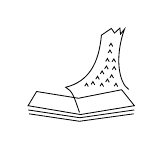
\begin{tikzpicture}[x=.45cm,y=.45cm,line width=.3pt]
\draw (0,0)--(.24,.4)--(1.42,.21)--(2.64,.45)--(3,0)--(1.48,-.25)--cycle;
\draw (0,-.12)--(1.46,-.34)--(3,-.12) (.03,-.23)--(1.45,-.44)--(2.98,-.23);
\draw (1.45,-.19)..controls (1.3,.25) and (1.25,.42)..(1.06,.52)
 ..controls (1.72,.68) and (2,1.21)..(2.07,1.99)
 --(2.35,2.18)--(2.44,2.05)--(2.59,2.19)--(2.61,2.02)
 --(2.72,2.16)..controls (2.43,1.35) and (2.57,.63)..(2.84,.46);
\foreach \x/\y in {1.6/.55,1.78/.6,1.91/.75,2.04/.9,2.16/1.04,2.19/1.25,2.26/1.49,2.29/1.68,2.03/.55,2.19/.67,2.31/.79,2.38/1.02,2.37/1.24,2.43/.55}
{\draw (\x,\y)--++(.05,.08)--++(.05,-.09);}
\end{tikzpicture}}
% crop-candidate: scan 14
NAGOYA UNIV.

名古屋大学内 \quad \unsure{日本郵便}\\
20.12.77 \quad NAGOYA DAIGAKUNAI \quad 0,340\\
H1208 \quad JAPAN

Professeur Alexandre Grothendieck\\
34700 Villecun (Lod\=eve)\\
\uline{FRANCE}

VIA AIR MAIL\\
PAR AVION

PAR AVION\\
航空郵便

\handwritten{\unsure{340|3X0}}

\handwritten{$\{\lambda,\lambda^{-1}\}\quad|\lambda|\ne1$\quad donc $\lambda\ne\lambda^{-1}$ i.e. $\lambda^2\ne1$ i.e. $\lambda\ne\pm1$ i.e. $\alpha\ne\pm2$}

\handwritten{$\lambda+\lambda^{-1}=\alpha$\qquad\deleted{\unsure{pte|qqc|tel que}} $\alpha\notin[-2,+2]$}
\[
\handwritten{\begin{aligned}
\alpha^2-4\qquad &\unsure{\nLeftrightarrow|\not\Leftarrow}\lambda\bar\lambda=1\\
&\bar\lambda=\lambda^{-1}\\
&\lambda+\lambda^{-1}\ \text{\uline{réel}}
\end{aligned}}
\]
% archive sheet number: 13
\scanpage{16}

\mspage{\handwritten{1}}

\begin{flushright}Les Aumettes 15.4.1984\\\end{flushright}
Dear Lipman Bers,\\

Together with Yves Ladegaillerie (a former student of mine) we are running a microseminar \deleted{\unsure{O|o}}on the Teichmüller spaces and groups, my own motivations coming mainly from algebraic geometry, and Ladegaillerie\unsure{(|'}s from his interest in the topology of surfaces. Lately we have met with a problem which I would like to submit to you, as I understand you are the mai\unsure{n} expert on Thurston's hyperbolic geometry approach to Teichmüller space. Before stating the specific problem on hyperbolic ``pants'' (which things boil down to\handwritten{)}, \deleted{L}\handwritten{l}et me tell you what we are really after.

Assuming given a compact oriented surface with boundary $X_0$ \deleted{\unsure{now}} as a reference-surface for constructing the Teichmüller-type spaces, of genus $g$ and with \quad ``holes'' (satisfying $\deleted{\unsure{2}}2g-2+\handwritten{\nu}>0$), my primary interest is in the more ``algebraic'' version of Teichmüller space, corresponding to the question of classifying algebraic non singular curves over $\underline{\mathrm C}$, of genus $g$, with a system of \quad points (all distinct) given on $X$, together with a ``Teichmüller rigidification'' of $(X,S)$ namely a homotopy equivalence between $X_0$ and $X\backslash S$. I'll denote this space, homeomorphic to $\underline{\mathrm C}^{d}$ (where $d=3g-3+\handwritten{\nu}$), by $\overset{\handwritten{\sim}}{\mathrm M}_{\handwritten{g,\nu}}$ (the tilda suggesting that it is the universal covering of a finer object I am still more interested in, namely the algebraic variety (or rather ``multiplicity'', or ``stack'' in the terminology of Mumford-Deligne) of modul\deleted{\unsure{a}}i for algebraic curves of type $(\handwritten{g,\nu})$. Thurston however considers a different modular space, where algebraic curves with a given system of points are replaced by compact conformal oriented surfaces \uline{with boundary}, giving rise to a modular space $\overset{\handwritten{\sim}}{\mathrm{MB}}_{g,\handwritten{\nu}}$ (where the letter B recalls that we are classifying structures with boundary) homeomorphic to $\underline{\mathrm C}^{d}\mathbin{\mathrm x}(\underline{\mathrm R}^{*+})^{\handwritten{\nu}}$, where the extra factor \deleted{$\unsure{\underline{\mathrm C}^{d}}$} corresponds to the extra parameters introducing through the existence of the boundary, namely the length's of the \deleted{various} components of the boundary with respect to the canonical hyperbolic structure on the given surface. Our interest is in pinpointing the precise relationship between the two modular spaces

The obvious idea here is to consider the case of an algebraic curve with \handwritten{$\nu$} points given as a limit-case of a \inserted{compact} conformal surface with boundary, when all the lengths $\deleted{1}\handwritten{\ell}_{\mathrm i}$ \deleted{\unsure{6}}of the components of the boundary tend to zero. Therefore, it looks suitable to consider both modular spaces above as imbedded in a larger third one, which corresponds to the same modular problem as in Thurston's theory, except that we allow the ``bo\deleted{\unsure{p}}undary'' to have some components reduced to just one point, in the neighbourhood of which X is just a conformal surface without boundary, but with a given point
% archive sheet number: 15
\scanpage{17}

\mspage{\handwritten{2}}

(viewed as a component of such a ``generalised boundary''). We now should \deleted{should} get a modular space for ``compact conformal oriented surfaces with generalized boundary'' (of type $g,\handwritten{\nu}$ and rigidified via $X_0$), call it $\overset{\handwritten{\sim}}{\mathrm{MB}}_{\handwritten{g,\nu}}$, homeomorphic to $\underline{\mathrm C}^d\mathbin{\mathrm x}(\underline{\mathrm R}^{\deleted{\unsure{*}}+})^{\handwritten{\nu}}$, where now the second factor corresponds to \deleted{\unsure{th}} the ``parameters'' $\handwritten{\ell_i}$, which are allowed to take also value 0 (which means that the corresponding component of the generalized boundary is just one point). Thus $\overset{\handwritten{\sim}}{\mathrm{MB}}_{\handwritten{g,\nu}}$ appears as a variety with boundary (in the topological sense - in the real analytic sense, the ``boundary'' admits ``corner-like'' points obviously), and $\overset{\handwritten{\sim}}{\mathrm M}_{g,\handwritten{\nu}}$ appears as a part of the boundary.

My interest is in a better geometric understanding of the situation, which should be ``intrinsic'' namely not depend on any particular choice of a surgical decomposition of the reference surface $X_0$ into ``pants'', used in order to describe in a handy way \deleted{the} standard ``coordinate\deleted{\unsure{s}} functions'' on the modular space $\overset{\handwritten{\sim}}{\mathrm{MB}}_{g,\handwritten{\nu}}$. There appears to be a geometrically meaningful retraction of $\overset{\handwritten{\sim}}{\mathrm{MB}}_{g,\handwritten{\nu}}$ \deleted{$\unsure{\mathrm M}$} upon $\overset{\handwritten{\sim}}{\mathrm M}_{g,\handwritten{\nu}}$ (commuting to the operations of the Teichmüller modular group), the fibers being homeomorphic to $(\underline{\mathrm R}^{+})^{\deleted{\unsure{I}}\handwritten{\nu}}$ - more specifically, I expect the semi-group $(\underline{\mathrm R}^+)^{\mathrm I}$ (where I is the set of indices for the ``holes'' of $X_0$) to act on $\mathrm{MB}$ in a natural way, with free action of the subgroup $(\mathrm R^{+\deleted{\unsure{x|*}}})^{\handwritten{\nu}}$ upon $\overset{\handwritten{\sim}}{\mathrm{MB}}^{\mathrm o}$, in such a way that $\overset{\handwritten{\sim}}{\mathrm M}$ is just the quotient of $\overset{\handwritten{\sim}}{\mathrm{MB}}$ by this action (or of $\overset{\handwritten{\sim}}{\mathrm{MB}}^{\mathrm o}$ by the action of the \deleted{\unsure{acting}} corresponding subgroup), and that \deleted{\unsure{e}}each fiber \inserted{$\mathrm F$} is isomorphic to $(\underline{\mathrm R}^+)^{\mathrm I}$ by the choice of any ``origin'' in $\mathrm F\handwritten{\cap}\overset{\handwritten{\sim}}{\mathrm{MB}}^{\mathrm o}$.

Of course, ``comput\deleted{\unsure{i|a}}\unsure{a|i}nnally'', in terms of a decomposition of $X_0$ into pants, the idea of such an operation is pretty obvious - namely letting the components $\handwritten{\lambda}_{\mathrm i}$ of $\handwritten{\lambda\in}(\underline{\mathrm R}^+)^{\mathrm I}$ act as a ``multiplier'' on the corresp\inserted{ond}ing coordinate $\deleted{\unsure{h}}\handwritten{\ell}_{\mathrm i}$. However, it is not clear that this operation is intrinsic - and if it were intrinsic, an intrinsic geometric description would still be \deleted{\unsure{in|is}} desired.

Of course, in the description of the situation proposed above, the retraction of $\overset{\handwritten{\sim}}{\mathrm{MB}}$ upon $\overset{\handwritten{\sim}}{\mathrm M}$ is obtained by multiplying with the 0 multiplier (all $\handwritten{\lambda}_{\mathrm i}$ are 0). Now there is a direct geometrical description of \deleted{this} a retraction, by hyperbolic surgery. Namely, for any \inserted{compact} conformal surface of type $g,\handwritten{\nu}$ with generalized boundary, let's ``fill in'' the holes which correspond to ordinary components of the boundary, which are riemanian oriented circles, by ``gluing in'' the cones on these circles (which are canonically endowed with a conformal structure, using the riemanian structure on the given circles). Thus we get a ``functor'' from \inserted{compact} conformal surfaces with generalized boundary \deleted{\unsure{t}}(of type $g,\handwritten{\nu}$) to compact conformal surfaces \uline{without boundary}, endowed with a system of \handwritten{$\nu$} points (making up a
% archive sheet number: 16
\scanpage{18}

\mspage{\handwritten{3}}

``wholly degen\deleted{\unsure{r}}erate'' generalized boundary). When we throw in the rigidifications and go over to isomorphism classes, this should give the desired retraction. However, the geometric situation is a lot richer still, as the compact surface without boundary obtained through surgery is endowed, not only with a system of \handwritten{$\nu$} points, b\deleted{\unsure{y}}ut moreover with a system of mutually disjoint \uline{discs} around these points. The shape of these discs is by no means arbitrary - we'll say that a system of discs around \handwritten{$\nu$} points on a compact \inserted{conformal} surface $X^{\wedge}$ without boundary is ``admissible'', if the situation can be obtained as above (up to isomorphism) from surgery, starting with a compact conformal surface $X$ w\deleted{\unsure{j}}ith bo\uline{u}ndary. (NB Among the given``discs'', we should allow \deleted{\unsure{s}}that some should be reduced to their center - we'll call them ``degenerate''\handwritten{)}The condition of admissibility can be expressed intrinsically, by stating that \deleted{the} for every non-degenerate component $\Gamma_{\mathrm i}$ of the system of boundaries of those discs, the two operations we got of the standard circle group (of complex numbers of module 1) upon $\Gamma_{\mathrm i}$, by using the fact that it is (on the one hand) the boundary of the disc $D_{\mathrm i}$, and (on the other hand) that it is a component of the boundary of the hyperbolic surface $X^\wedge\backslash(\handwritten{\bigcup_{\mathrm j}}D^{\mathrm o}_{\mathrm j})$, should be the same. \margin{\handwritten{!}} When $X^\wedge$ and the points $s_{\mathrm i}$ on $X^\wedge$ are given, the possible \inserted{admissible} systems of discs around the points $s_{\mathrm i}$ depend on \handwritten{$\nu$} parameters - and the first idea which flips to mind to give a more precise meaning to these ``parameters'', is to view them as being the``radii'' of those discs. But then we'll have to define what we mean by these !

The idea here is that, when we have a conformal disc $D$ and an inter\deleted{\unsure{a}}ior point $s$ of $D$, then $D$ may be viewed as canonically embedded in \deleted{\unsure{h}}the tangent space $T_{\mathrm s}$ to $D$ at $s$, as th\^{e} ``unit disc'' at $s$. Thus, in the situation above of an\deleted{\unsure{just}} admissible system of discs $(D_{\mathrm i})_{\mathrm i\handwritten{\in}\mathrm I}$ around $(s_{\mathrm i})_{\mathrm i\handwritten{\in}\mathrm I}$, for every $s_{\mathrm i}$ corresponding to a non-degenerate $D_{\mathrm i}$, we get a canonical disc
\[
\handwritten{\Delta}_{\mathrm i}\handwritten{\subset} T_{s_{\mathrm i}}
\]
in the tangent space - and of course, for degenerate $D_{\mathrm i}$, we'll take $\handwritten{\Delta}_{\mathrm i}$ to be degenerate too. The discs we get in a\deleted{g} given $T_{s_{\mathrm i}}$ (for a fixed system $(s_{\mathrm i})$, and a variable \inserted{admissible} system of discs around these $s_{\mathrm i}$) are all discs in the strict euclidean sense, given by an unequality
\[
\handwritten{|}z\handwritten{|}\ \handwritten{\leqslant}\ r_{\mathrm i}\quad,
\]
where $z\handwritten{\mapsto|z|}$ denotes some hermitian metric on $T_{s_{\mathrm i}}$ compatible with the conformal structure - this metric being \deleted{defined}\inserted{\handwritten{unique}} up to a scalar factor. the set \inserted{$\mathrm R_{\mathrm i}$} of all those possible discs (the non-degenerate one\handwritten{s}\deleted{\unsure{,}}, say) may be viewed in a natural way as a ``torsor'' (= principal homogeneous space)
% archive sheet number: 17
